%%%%%%%%%%%%%%%%%%%%%%%%%%%%%%%%%%%%%%%%%%%%%%%%%%%%%%%%%%%%%%%%%%%%%%%%%%%%%%%%
%2345678901234567890123456789012345678901234567890123456789012345678901234567890
%        1         2         3         4         5         6         7         8

\documentclass[letterpaper, 10 pt, conference]{ieeeconf}  % Comment this line out
                                                          % if you need a4paper
%\documentclass[a4paper, 10pt, conference]{ieeeconf}      % Use this line for a4
                                                          % paper

\IEEEoverridecommandlockouts                              % This command is only
                                                          % needed if you want to
                                                          % use the \thanks command
\overrideIEEEmargins
% See the \addtolength command later in the file to balance the column lengths
% on the last page of the document

\usepackage{url}
\usepackage{circuitikz}
\usepackage{siunitx}
\usepackage{csquotes}
%\usepackage[babel=true]{csquotes}
%\sisetup{output-decimal-marker = {,}}
%\usepackage{subcaption}
\usepackage{mathtools}
\usepackage{graphicx}
\usepackage{dblfloatfix}
\usepackage{kantlipsum}
%\usepackage[colorinlistoftodos]{todonotes}
%\usepackage{appendix}
%\renewcommand{\appendixpagename}{Annexes}
%\renewcommand{\appendixtocname}{Annexes}


\usepackage{listings}
\usepackage[colorlinks=true, allcolors=black]{hyperref}
\usepackage{cleveref}

% The following packages can be found on http:\\www.ctan.org
%\usepackage{graphics} % for pdf, bitmapped graphics files
%\usepackage{epsfig} % for postscript graphics files
%\usepackage{mathptmx} % assumes new font selection scheme installed
%\usepackage{times} % assumes new font selection scheme installed
%\usepackage{amsmath} % assumes amsmath package installed
%\usepackage{amssymb}  % assumes amsmath package installed

\title{\LARGE \bf
Study of performance variability of LoRa/LoRaWAN telecommunication systems
}

%\author{ \parbox{3 in}{\centering Huibert Kwakernaak*
%         \thanks{*Use the $\backslash$thanks command to put information here}\\
%         Faculty of Electrical Engineering, Mathematics and Computer Science\\
%         University of Twente\\
%         7500 AE Enschede, The Netherlands\\
%         {\tt\small h.kwakernaak@autsubmit.com}}
%         \hspace*{ 0.5 in}
%         \parbox{3 in}{ \centering Pradeep Misra**
%         \thanks{**The footnote marks may be inserted manually}\\
%        Department of Electrical Engineering \\
%         Wright State University\\
%         Dayton, OH 45435, USA\\
%         {\tt\small pmisra@cs.wright.edu}}
%}

\author{Jovicic Nikola}% <-this % stops a space
%\thanks{*This work was not supported by any organization}% <-this % stops a space
%\thanks{$^{1}$Polytechnic Faculty of Mons,
%        University of Mons, 7000 Mons, Belgium}%
%\thanks{$^{2}$P. Misra is with the Department of Electrical Engineering, Wright State University,
%        Dayton, OH 45435, USA
%        {\tt\small p.misra at ieee.org}}%
%}


\begin{document}



\maketitle
\thispagestyle{plain}
\pagestyle{plain} % Put plain when the article is finished


%%%%%%%%%%%%%%%%%%%%%%%%%%%%%%%%%%%%%%%%%%%%%%%%%%%%%%%%%%%%%%%%%%%%%%%%%%%%%%%%
\begin{abstract}

%In the scope of the MAB1 project of the FPMS ... This paper presents the study of a LoRa/LoRaWAN telecommunication system in an urban environment. The first part will present the experimental material used for this study some technical informations about them. A map will also show the location of each device in the experiment area.

This report was written by a student in the frame of the MAB1 project of "Multimedia and Telecommunications" at the FPMS (Facult\'e Polytechnique de Mons) of UMons in Belgium. This paper presents a study of the variability of reception of a LoRa/LoRaWAN wireless communication system in an urban environment, in the city of Mons. To perform the study, 8 LoRa emitters have been placed in the area and 2 receiving gateways. The emitters were sending every 10 minutes temperature, relative humidity and pressure measurements from their location. This study shows that the obstacles of urban environment and the distance between the emitter and the receiver affect greatly the quality of the transmission. There is also a link between the RSSI and the SNR, which appears to be exponential and positive, and the limiting factor of a LoRa transmission seems to be the SNR, not the RSSI. In addition, the temperature, coupled with humidity, influences negatively the transmission. The pressure, however, doesn't seem to impact the communication.

\end{abstract}

%%%%%%%%%%%%%%%%%%%%%%%%%%%%%%%%%%%%%%%%%%%%%%%%%%%%%%%%%%%%%%%%%%%%%%%%%%%%%%%%
\section{Introduction}

The Internet of Things is the the connection of physical devices to the Internet and between themselves \cite{c1}. Such devices are usually embedded electronics or sensors that send a smaller amount of data than classical Internet applications on smartphones, tablets or computers. Also, the battery lifetime is an important factor to consider. Specific protocols to the IoT world exist (CoAP, Sigfox, ZigBee, AMQP, ...\cite{c3}\cite{c17}) and one of them is LoRaWAN (MAC layer protocol in the OSI model). This protocol allows low-speed communications, using radio frequencies and for devices with limited access to power, both electrical and computational \cite{c4}. The physical implementation is called LoRa. It uses Chirp Spread Spectrum (CSS) modulation in order to send data up to 15 km (in a rural environment) \cite{c5}\cite{c19}. Data sent by the emitters is received by gateways that will send the information on the Internet. The slope of the instantaneous  frequency of the chirp depends on a spreading factor SF. Two symbols sent with different SF are quasi-orthogonal and do not interfere with each other. The higher the SF, the greater is the transmission distance but the slower is the communication (smaller bit rate) \cite{c5}.

This project aims to implement a LoRa telecommunication system by placing emitters in and near the city of Mons. It analysis the performance variability of the transmissions (from the different emitters to the receivers). The goal is to determine which are the most influencing factors on the communication (distance, temperature, relative humidity, ...) and to establish the possible existence of a correlation between the transmission and these factors.

\section{Methodology}

\begin{figure}[ht!]
\centering
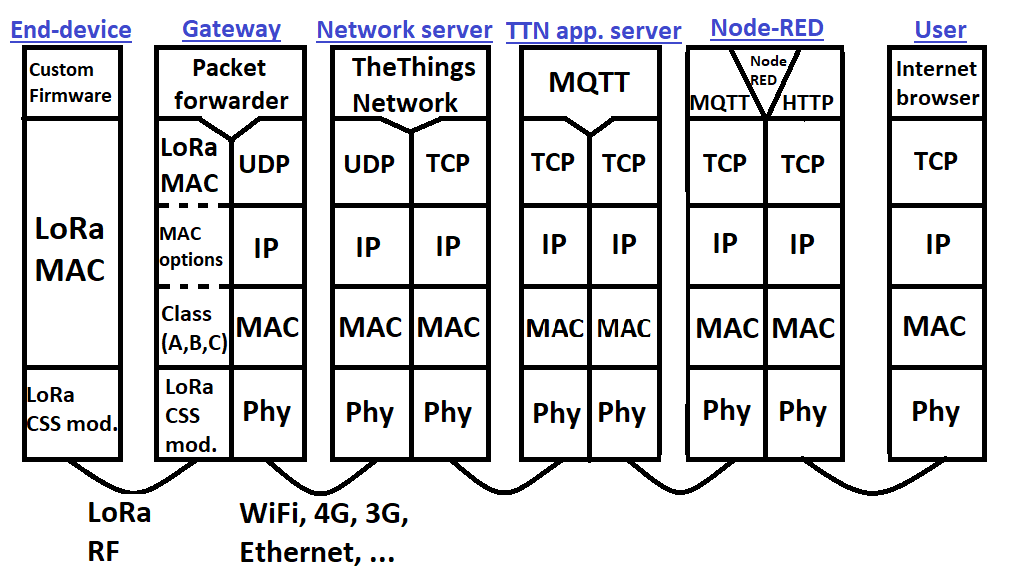
\includegraphics[scale=0.32]{tx_chain.png}
\caption{Complete transmission chain for data collection}
\label{chain}
\end{figure}

The practical implementation for collecting the data is shown in figure \ref{chain}. The end-device, before accessing the IoT network of "TheThingsNetwork", is activated through the  OTAA (Over-the-Air Activation) process. The device and the network server exchange keys and unique identifiers that are used later by the device for transmitting its data to our own application server \cite{c6}. This process is mandatory to identify the device and allow it accessing the network.

After this activation process, the device can broadcast its data (encrypted and with a checksum to verify its integrity at the reception) to any compatible LoRa receiver . These receivers are called gateways and they forward the packets to the network server of TTN (if the device is identified on this network). Then, the packets are verified (integrity check) and decrypted by the TTN application server before being sent to the user's application server (here, Node-RED). Finally, the user can see the data in Node-RED from his browser and can also export the data to a text file.

\subsection{Emitters}

The static devices that have been used for this project comprise a \textit {lopy MicroPython} development board using LoRa for radio transmission and a \textit{Pysense} board on which the \textit{lopy} is connected and that senses temperature, relative humidity and pressure inside the case. The whole system runs on a lithium battery (AA size). The case of the static devices is 3D-printed and conceived in such a way that water droplets and humidity should not enter inside the area containing the electronic components. The emission antenna is standard and is not calibrated. The payload (5 bytes) sent by each device is composed of the temperature (10 bits), relative humidity (8 bits) and barometric pressure (12 bits) sensed by the \textit{Pysense} module. The battery level (10 bits) was also sent in the payload (only to monitor the variation of the battery level). The nodes 6\_02 and 6\_03 were placed on the $4^{th}$ of April 2019 and the nodes 7\_01, 7\_02 and 8\_01 were placed on the $5^{th}$ of April 2019. The devices 6\_01, 8\_03 and 8\_04 have been placed 2 weeks before the end of data collection (respectively 25.04, 26.04 and 28.04), which has been concluded on the $6^{th}$ of May 2019.

The choice of the spreading factor for emitting the packets is important, as higher spreading factors imply a longer time on air and the duty cycle limitation of 1\% must not be exceeded \cite{c13}. To avoid this situation, the lower spreading factors were chosen more often than the higher ones. The emitters were programmed in such a way that for 63 packets sent, 32 will be sent with a SF7, 16 with a SF8, 8 with a SF9, 4 with a SF10, 2 with a SF11 and 1 with SF12. It is not a probabilistic drawing but a way to send packets with different SF, without spending excessive time in the air \cite{c2}. The distribution is shown in the figure \ref{sf_packet_count}, for the whole data.

\begin{figure}[ht!]
\centering
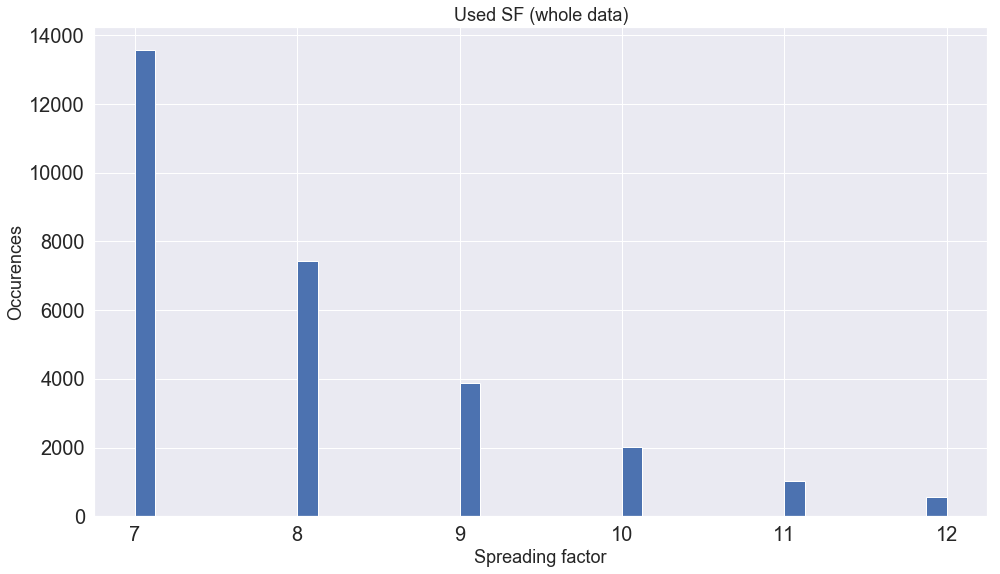
\includegraphics[scale=0.24]{sf_count.png}
\caption{SF used to send packets}
\label{sf_packet_count}
\end{figure}

\subsection{Gateways}

There were two receivers with different hardware at two different locations. The first one is on the roof of the UMons building "La cit\'e Houzeau". The model is a \textit{Kerlink Wirnet Station} with a specified reception sensitivity level as low as -141 dBm \cite{c7}. Its identifier is "eui-0000024b08030186". The second receiver is inside a building, at the street of "Joncquois", ground level. This model is a \textit{RAK831} using a \textit{Semtech} chip that allows reception sensitivity levels of -124 dBm for a spreading factor 7 (fast transmissions) and -137 dBm for a spreading factor 12 (slow transmissions but more resistant to noise) \cite{c8}. Its identifier is "iotlab-rpi-03".

\subsection{Emitter and receiver positions}

\begin{figure}[ht!]
\centering
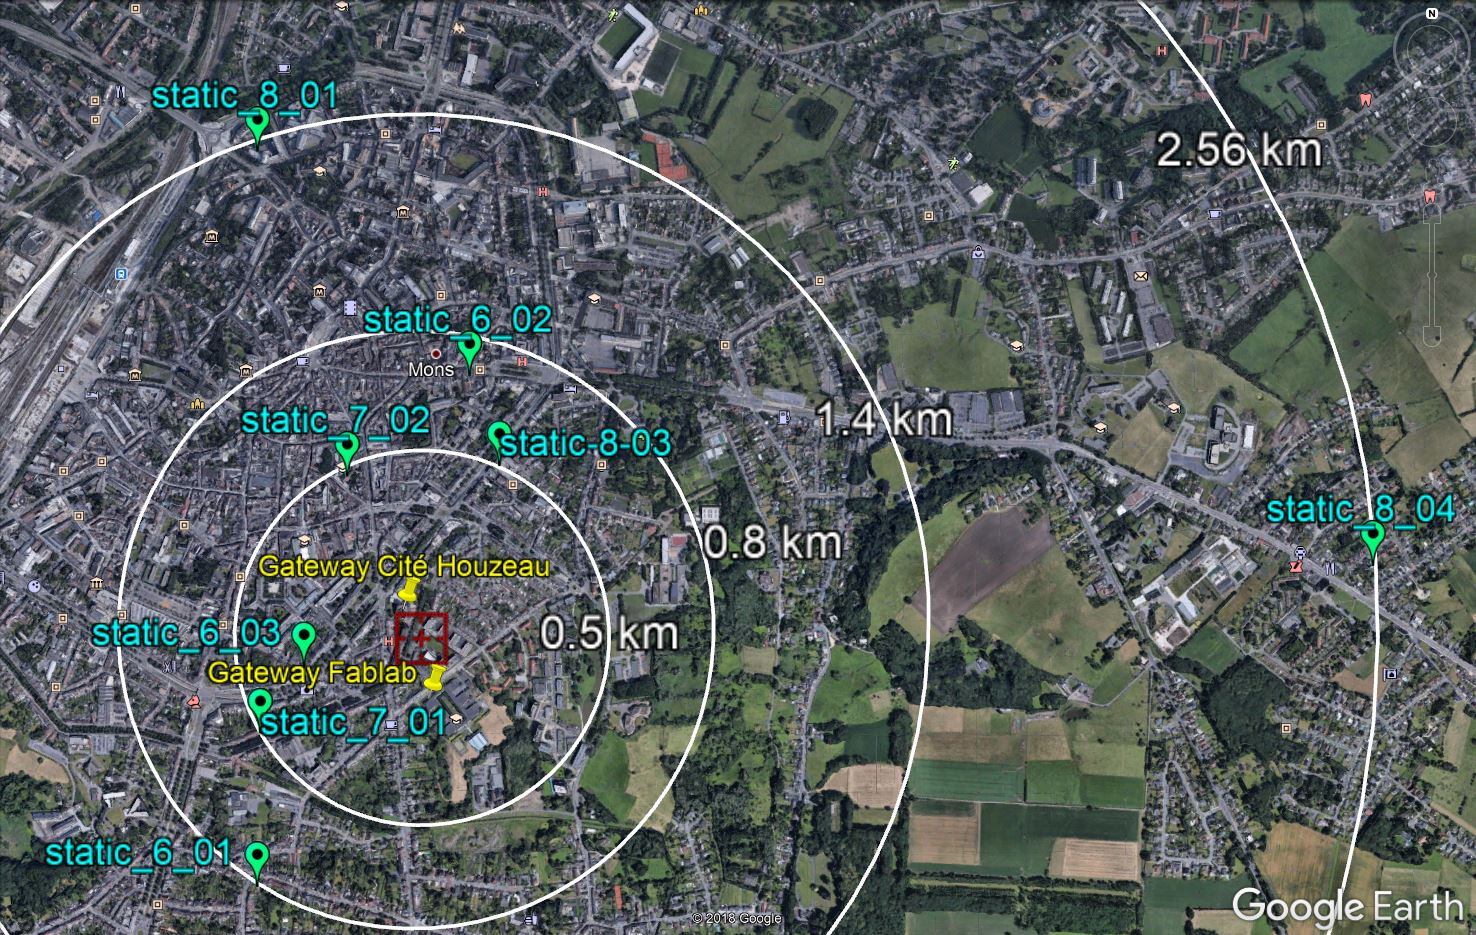
\includegraphics[scale=0.22]{location_map.JPG}
\caption{Geographical location of emitters (blue) and receivers (yellow) (Image taken using Google Earth Pro)}
\label{location_map}
\end{figure}

The experiment has been conducted in the vicinity of the city of Mons (see map on figure \ref{location_map}). Except for the device 8\textunderscore{}04, the emitters and the receivers were placed in urban environment. The emitters 6\textunderscore{}01 and 7\textunderscore{}02 were the only emitters to be placed indoor. The rest of the emitters were placed outdoor. The white circles represent the approximate distance from the receivers (in fact the middle between the two gateways is represented by the red square).

% Image of the map showing the emitters and receivers locations in Mons

\subsection{Data analysis tools}

Data analysis has been performed using Python 3 with Spyder and Jupyter.

\section{Results and discussion}

This section presents the data collected from the experiment and some general trends that have been seen in the transmissions. The first will presents the difference in data reception per device and per gateway. The second point focuses on the distance between the emitters and the receivers, the topology of the area and the presence of obstacles. The next points focus on technical (RSSI and SNR) and environmental parameters (temperature, relative humidity and pressure) and establish their impact on the transmission.

The database provided the following information : timestamp (up to the ns), device ID (the name of the emitter), device eui (unique identifier on TTN), gateway ID (the name of the gateway that received the packet), counter (number that increments by one unit each time a new packet is sent by the emitter), frequency (in MHz), data rate (SF and bandwidth), coding rate, RSSI, SNR, battery level, humidity, pressure and temperature
% Present trends
% We are going to present this, that, ... (quelques lignes pour expliquer au lecteur ce qu'il va lire.

\begin{figure*}[t]
\centering
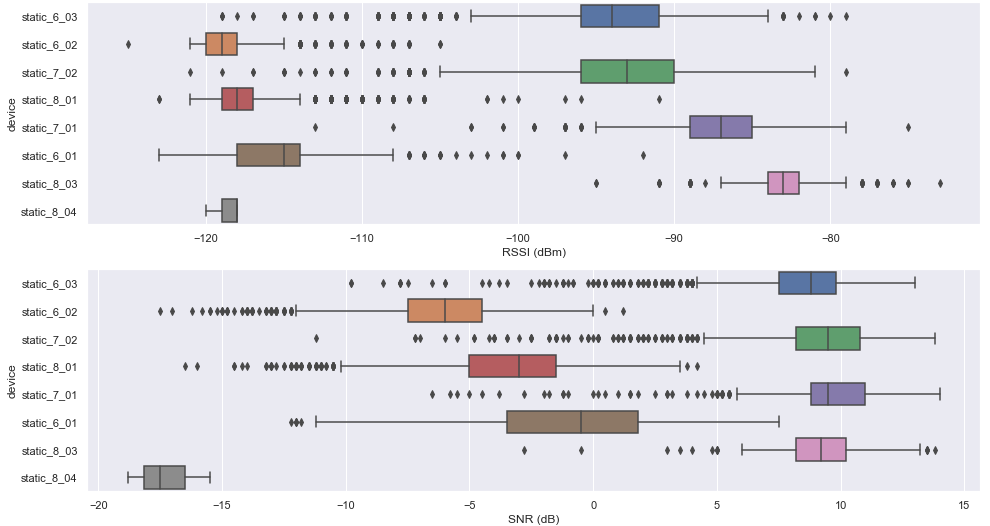
\includegraphics[scale=0.48]{boxplot.png}
\caption{RSSI (top) and SNR (bottom) dispersion at the gateway eui-0000024b08030186 \cite{c2}}
\label{boxplot}
\end{figure*}

\subsection{Data reception and dispersion}

Tabe \ref{table_packets} in the appendix shows the number of packets that were received by the two gateways. It is clear  that the gateway eui-0000024b08030186 at the top of the building "Cit\'e Houzeau" received most of the packets from the emitters. Almost 75\% of the successful packets were received by this gateway. This is explained by the height and the fact that the gateway was placed outside (not inside a building).
%This implies that the higher the receiver is, the better is the reception. This is also confirmed by the case of the other receiver, which is at the ground level, inside a building surrounded by many other buildings and houses, who could not receive as much packets.

Figure \ref{boxplot} shows the dispersion of the RSSI (Received Signal Strength Indication) and SNR (Signal to Noise Ratio) for each device at the gateway eui-0000024b08030186. It appears that the behaviour of each device is different and data dispersion is also not identical for each emitter. %This same figure also  shows that packets with a lower RSSI tend to have a lower SNR. Say : en moyenne, ce graphique que ...
The device 8\_04 is a particular case, because it has only successfully sent 3 packets and therefore, has no dispersion in the data. It will be explained later in this article ("\textit{C. Distance between emitters and receivers}").

%A possible explanation of the dispersion is the placement of the emitters. Some of them are located in an area with a lot of buildings causing some screening effect (like 6\_02) and some of them are relatively far from the receivers (like 8\_01 or 8\_04).

\subsection{FER (Frame Error Rate)}

The FER can be computed by looking at the "counter" value of the received packet at the gateway. Each time a packet is sent by the device, its counter increments by one unit, which means that in an ideal case the values of the counter always follows an arithmetic progression of common difference equal to 1. In practice, every packet that is sent is not necessarily received. The table \ref{table_fer} shows the percentage of the FER on each link. Where there is 100\% it means that no packet has been transmitted on this link.

\begin{table}[htbp]
\begin{center} 
\begin{tabular}{|c|c|c|}
  \hline
    dev$\setminus$gtw & eui-
0000024b08030186 & iotlab-rpi-03 \\
  \hline
  static\_6\_01 & 22.319\% & 100\% \\
  \hline
  static\_6\_02 & 49.1085\% & 100\%\\
  \hline
  static\_6\_03 & 3.5887\% & 33.9718\% \\
  \hline
  static\_7\_01 & 2.2207\% & 20.2839\% \\
  \hline
  static\_7\_02 & 3.0909\% & 98.1789\%\\
  \hline
  static\_8\_01 & 24.5774\% & 100\% \\
  \hline
  static\_8\_03 & 3.396\% & 36.5607\% \\
  \hline
  static\_8\_04 & 99.6774\% & 100\% \\
  \hline
  \end{tabular}
  \end{center}
 \caption{FER of each link\label{table_fer}}
\end{table}

A quick analysis of this table reveals that the receiver at Joncquois (iotlab-rpi-03) performs poorly at receiving packets from the emitters (contrary to the other gateway). When looking at devices that sent to both receivers (like 6\_03 or 7\_01), it clearly appears that the FER is higher at the Joncquois receiver (the one inside the building), meaning that something is deteriorating the quality of the transmission to this gateway. This is discussed in the following point.

\subsection{Distance between emitters and receivers}
Figure \ref{location_map} at the first page shows the location of the two receivers and the eight emitters. This figure also presents white circles that indicate the approximate distance from the receivers. By comparing the table \ref{table_packets} in the appendix, the figure \ref{boxplot} and the map, it is clear that the emitters closer to the receivers have higher RSSI and SNR values and have successfully sent a higher number of packets (6\_03, 7\_02, 7\_01 and 8\_03). Those who were further away from the receivers have a lower RSSI and SNR and are less successfull at transmitting packets correctly. It should be reminded that devices 6\_01, 8\_03 and 8\_04 have been placed 2 weeks before the end of data collection and it is normal that they have sent less packets than the other nodes. In practice, measurements show that under 800 m and in urban environment, RSSI and SNR remain in the higher range of values.

An important parameter to consider is the height at which the receivers are placed. The one at the top of the building Houzeau (eui-0000024b08030186) has received almost 75\% of the total number of received packets, and the indoor receiver (iotlab-rpi-03) at the  ground level has had much more trouble in receiving data, even though the two were not so far from each other (approximately 200 m). The higher receiver had less obstacles (trees, buildings, houses, ...) between it and the emitters. On the other hand, the Joncquois's receiver was inside a building at ground level, which meant that any signal arriving at this receiver was attenuated by the obstacles it had encountered (including the walls and the windows of the building)\cite{c16}. For instance, the number of packets sent by the node 6\_03 and received by the Houzeau's receiver was about 46 \% higher than at the Joncquois's receiver. The same observation can be seen at the node 7\_01, although the difference in reception is smaller (about 22\%). The hypothesis can be confirmed even more by the device 7\_02, which was emitting from inside a building, near a window. The table \ref{table_packets} clearly demonstrates that the Joncquois's receiver (inside a building at ground level) could not receive as much packets as the Houzeau's receiver (on the top of the roof). In fact, this is mostly due to the position of this device inside the city. The signal needed to go through the window, then travel the distance separating the emitter from the Joncquois's receiver and before it could reach the receiver, it was heavily attenuated by the obstacles on its path and the building where the receiver was located. The emitter 8\_01 has not been able to send a single packet to the Joncquois's receiver for the same reasons (position of the emitter relative to the receiver and obstacles in the path).
% Some study show that concrete and people attenuate wireless signals (add bibliography)

Not only the placement of the receivers is important, but so is the placement of the emitters. The device 6\_02 is roughly under 800 m of distance from the receivers, but table \ref{table_packets} and figure \ref{boxplot} indicate that it had some difficulties in sending its data properly. This is due to the fact that this particular emitter was placed in an area surrounded by a lot of buildings, which have considerably attenuated the signal. The farthest device (8\_04) that was placed near the end of the experiment only managed to send three packets properly ... The reason is that the emitter is hidden behind a hill, when looking from the receivers's perspective. Here, it is the topology of the landscape that had a major influence on the transmission.

These observations confirm a previous study made by a Swiss team in the Antarctic using mobile LoRa emitters, where the "\textit{varying terrain elevation is shown to be
the dominating factor influencing the propagation[...]}" \cite{c14}. This team could achieve up to 30 km of range between the base and the mobile emitters (using directional antennas) with a Line-of-Sight communication.

Another study has also highlighted the link quality degradation of indoor transmissions between buildings and confirms that indoor nodes closer to a door/window were able to send a stronger signal to the gateway \cite{c12}.

\subsection{Link between RSSI and SNR}

The RSSI and the SNR are two different values used to characterize the quality of the transmission. It is interesting to establish the existence of some kind of correlation between these two parameters.

The RSSI (Received Signal Strength Indicator) is a measurement of the power of the received signal from an antenna, usually expressed in dBm \cite{c9} \cite{c10}. The SNR (Signal-to-Noise Ratio) is a ratio that compares the power of the useful signal to the power of the background noise and interferers, usually expressed in dB. Above 0 dB, the useful signal has more power than the noise \cite{c11}. The RSSI will indicate the power of the received signal, but the SNR will tell the power of the useful signal.

The scatter plot of the RSSI as a function of the SNR on the whole data is shown on figure \ref{rssi_snr_general}. The best devices, with the highest number of successfully received packets and higher RSSI values tend to have a higher SNR. On the contrary, the weaker devices with a lower RSSI tend to have a lower SNR. The computation of the Pearson's linear correlation coefficient gives 0,874 (positively linear correlation).

\begin{figure}[hb!]
\centering
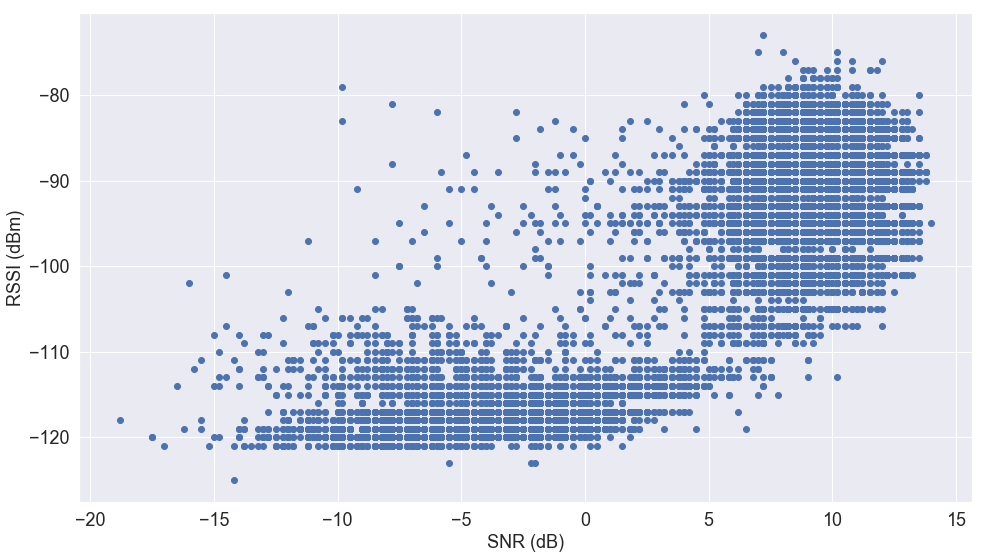
\includegraphics[scale=0.33]{general_rssi_snr_behaviour.png}
\caption{RSSI vs SNR at the Houzeau gateway (all devices)}
\label{rssi_snr_general}
\end{figure}

\subsection{The limiting factor of the transmission}

The fact that some packets were not properly received by the gateways means that some parameter(s) limit the reception of packets. In the scope of this project, it appeared that the SNR is the limiting factor.

The gateway Joncquois only received 68 packets from the emitter 7\_02, with the highest spreading factors only (10, 11 and 12 - see figure \ref{sf_7_02} in appendix). The sensitivity of this receiver is -137 dBm for SF12, but the lowest RSSI level was recorded at -108 dBm (29 dB above the sensitivty threshold). This means that the RSSI reception level didn't limit the reception of the packets, but it was the SNR. The lowest SNR value was recorded at -19.5 dB (with a RSSI level of -103 dBm) (see figure \ref{snr_limit} in the appendix).

For the device 8\_04, the lowest SNR value was -18.8 dB with a RSSI level of -118 dBm, at the Houzeau receiver.

Observations on other communications that present poor performances confirm that the RSSI sensitivity level of the receiver was never reached and that SNR values were always lower than -10 dB. Such low values of SNR are easily explained by the obstacles in the environment that attenuate the power of the signal (as explained previously).

\subsection{Frequency bands of a LoRa transmission}

The frequency of a LoRa transmission is at 868 MHz in Europe. In this experiment, 8 frequency bands, ranging from 867,1 MHz to 868,5 MHz, were available and almost equally used by the emitters under normal conditions (appendix - figure \ref{freq_count}). However, some transmissions had an issue at a specific moment in time. For instance, the node 6\_02 had a sudden packet delivery drop between the $12^{th}$ and the $17^{th}$ of April 2019 (appendix - figure \ref{6_02_freq_problem}). The analysis of the environmental parameters (temperature, relative humidity and pressure) showed no sudden change that could cause this issue. However, the analysis of the frequency band usage (figure \ref{602_freq_hist}) revealed that 3 frequency bands were much less used (867,5 MHz, 868,3 MHz and 868,5 MHz). This is confirmed by figure \ref{602_freq} in the appendix where those 3 frequencies were less used during this period (especially 867,5 MHz). A plausible hypothesis is that electromagnetic noise interfered with the LoRa transmission at this time (possibly other LoRa or Sigfox emitters). This phenomenon has also been observed on the node 7\_02 between the $8^{th}$ and $10^{th}$ of April at the Joncquois's gateway. This only remains a hypothesis, as no means of measuring the electromagnetic noise have been deployed in this project.

No similar problem has been observed during the rest of the experiment.

\begin{figure}[htbp]
\centering
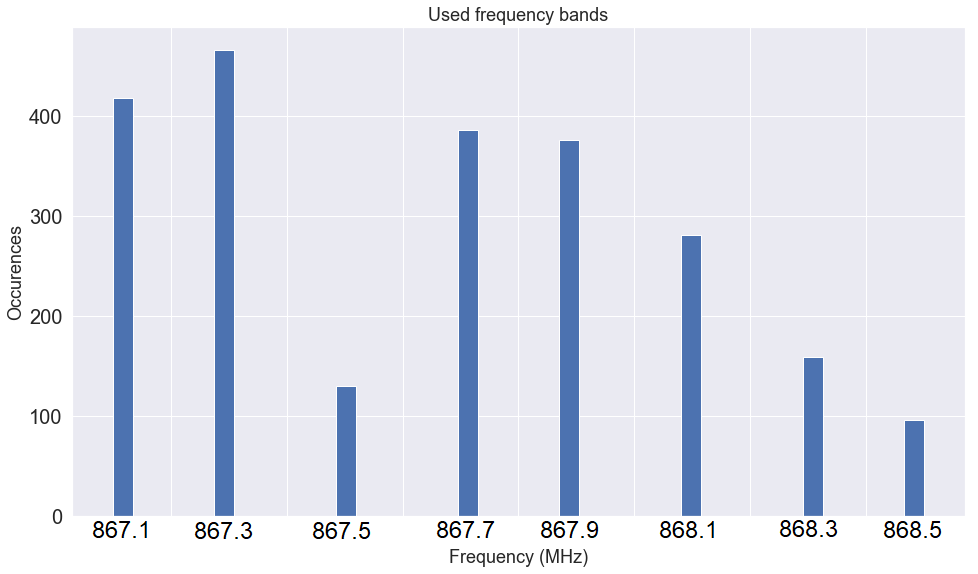
\includegraphics[scale=0.33]{6_02_freq_hist.png}
\caption{Histogram of the frequency bands used by 6\_02 during the experiment}
\label{602_freq_hist}
\end{figure}

\subsection{Impact of the temperature and relative humidity on the communication}

This subsection analyses the impact of the temperature and the relative humidity on the LoRa transmission. The analysis show global and daily variations (averaged over 24 hours).

The temperature evolution throughout the experiment was almost identical on every device (appendix - figure \ref{temp_all}). The device 7\_02 had the smallest variations (less than 10$^\circ$C), because it was inside a building. The device 7\_01 had undergone the largest variations in terms of temperature. The device 8\_03 had also large variations of temperature. During 24 hours, the temperature increases steeply from 5 to 13 o'clock and decreases smoothly afterwards. This can be observed on every device, every day (figure \ref{temp_24h_all}).

\begin{figure}[htbp]
\centering
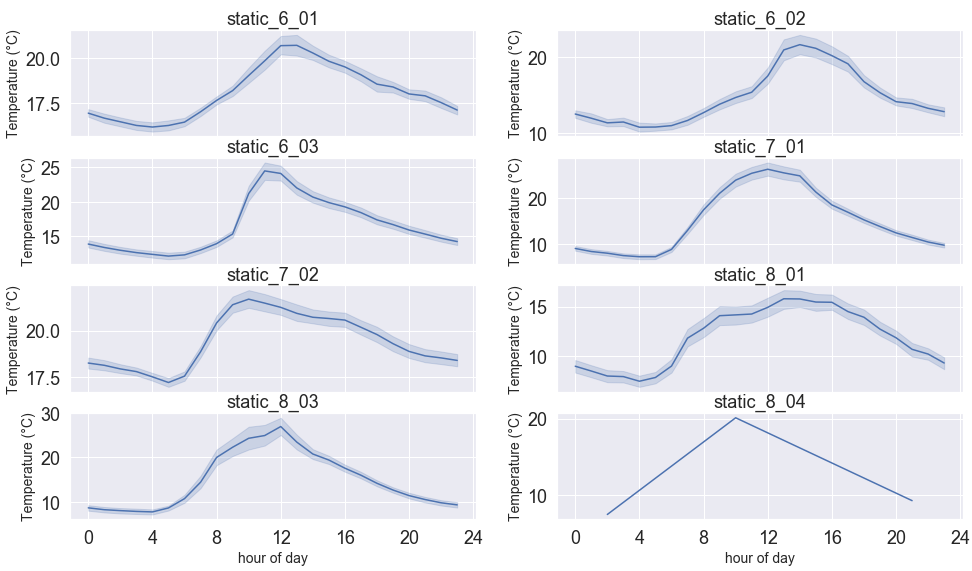
\includegraphics[scale=0.25]{02_temp_24h_all.png}
\caption{Temperature profile on each device (averaged values on 24 hours)}
\label{temp_24h_all}
\end{figure}

Evolution of the relative humidity was identical on emitters 6\_02, 6\_03 and 7\_02, with the last one having smaller variations. The largest changes of RH were observed on the node 7\_01 and, on average, values were the highest too. The device 8\_01 had a constant increase of humidity, from 25\% at the beginning of the experiment up to 75\% at the end of it. Other devices had no significant changes of RH (appendix - figure \ref{rh_all}).

\begin{figure}[htbp]
\centering
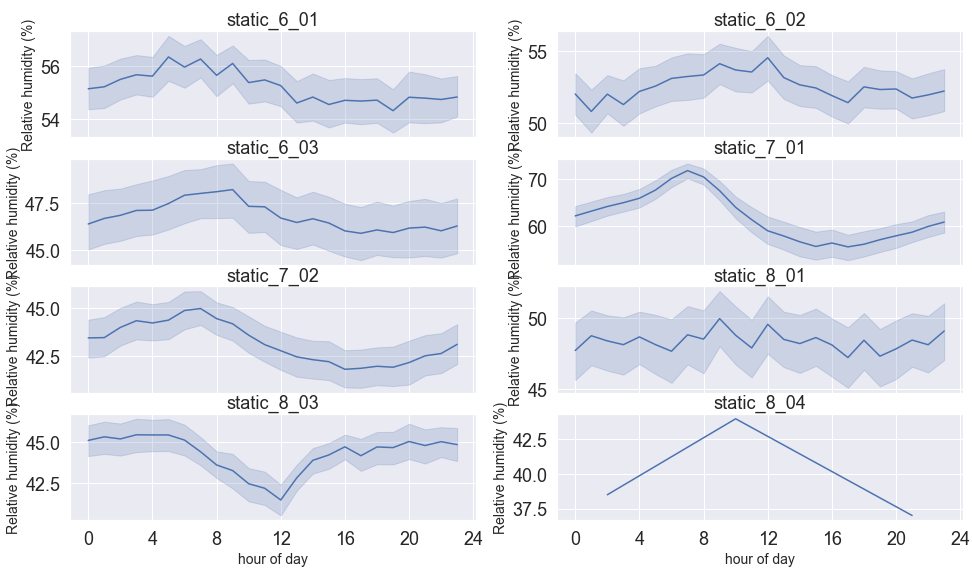
\includegraphics[scale=0.25]{01_rh_24h_all.png}
\caption{RH profile on each device (averaged values on 24 hours)}
\label{rh_24h_all}
\end{figure}

The average evolution of the SNR doesn't seem to be affected much by the environmental variations, but the average evolution of the RSSI is much more relevant (figure \ref{rssi_all_24}). During a full day (24 hours), the RSSI of emitters 6\_03 and 7\_01 fell by approximately 2 dB between 8 o'clock and 18 o'clock. For both devices, the temperatures were higher (over 25$^\circ$C) between these two moments of the day. The relative humidity, however, was different on both devices (figure \ref{rh_24h_all}), where 7\_01 has measured 60\% to 70\% of RH at this time. The other device measured 46\% to 48\% of RH. This demonstrates that the temperature is actually more influencing than the relative humidity, but coupled effects (high temperature and high humitidy) seem to produce a significant impact. According to Mrs V\'eronique Moeyaert, when an electronic equipment is put inside a box and this box is subject to high levels of relative humidity (inside humidity is above 50\%-60\%, without having necessarily condensation), if the sun rays hit directly the box then the temperature inside the housing will rise and can reach values up to 50$^\circ$C. This means that if the LoRa emitters have been exposed to humidity and directly to the sun, the transmission's RSSI has been affected. The fact that a LoRa transmission is affected by the temperature has been proved by a previous study, led by Austrian researchers who showed that a rising temperature from 10$^\circ$C to 40$^\circ$C lowered the RSSI by 3 dB \cite{c15}.

The emitter 7\_02 had minor variations in both parameters because it was protected inside the building from the external variations and its RSSI remained relatively constant. This indoor device proves that a controlled environment stabilises the quality of the transmission.

\begin{figure}[htbp]
\centering
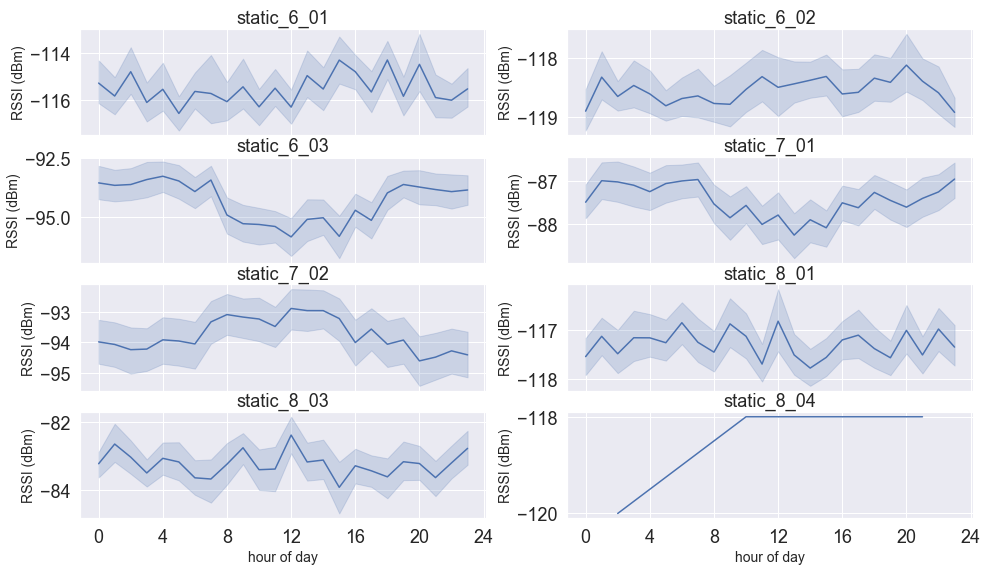
\includegraphics[scale=0.245]{rssi_all_24h.png}
\caption{RSSI of packets received at Houzeau gateway (24 hours)}
\label{rssi_all_24}
\end{figure}

%The average evolution of the temperature during a day can be seen at the figure \ref{temp_avg_24h}, which is taken from the device 6\_03 and describes perfectly the curve that can be observed on every device. The temperature rises steeply between 6 and 12 o'clock and decreases smoothly afterwards. The range of values goes from 8$^\circ$C to 28$^\circ$, measured directly at the emitters.

%\begin{figure}[htbp]
%\centering
%\includegraphics[scale=0.285]{rssi_snr_24h_603.JPG}
%\caption{Average evolution of the RSSI (left) and SNR (right) in a day }
%\label{rssi_snr_avg}
%\end{figure}

%The figure \ref{rssi_snr_avg} shows the general behaviour of the RSSI (left) and SNR (right) during 24 hours. It appears that the RSSI loses 2dB to 3dB of power between 6 and 18 o'clock. The SNR values have fluctuations of about 1 dB. The temperature definitely attenuates the signal received at the gateway, but doesn't seem to lessen the SNR. Instead, this ratio fluctuates



\subsection{Impact of the pressure on the communication}

\begin{figure}[htbp]
\centering
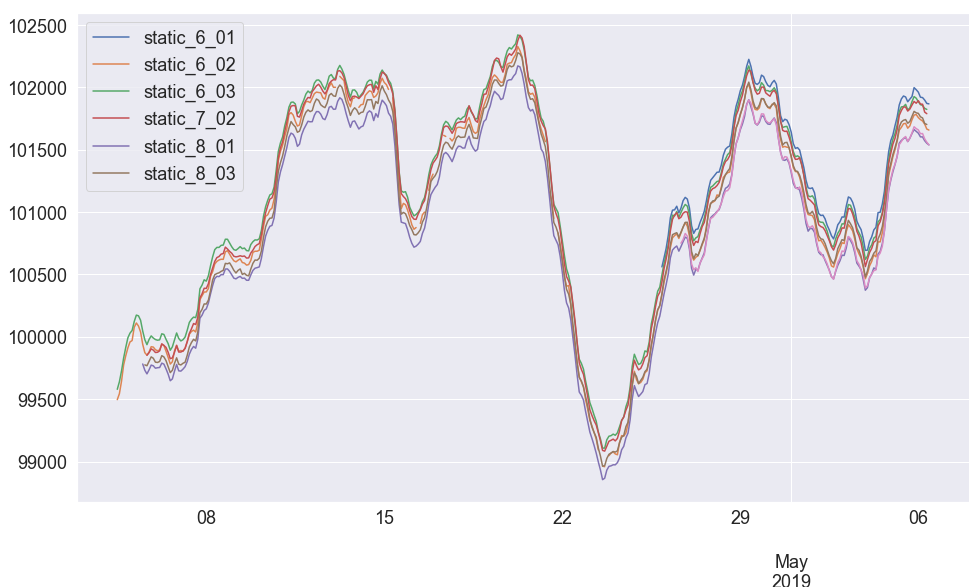
\includegraphics[scale=0.245]{pressure_general.png}
\caption{Evolution of the atmospheric pressure during the experiment (31 days)}
\label{pressure_general}
\end{figure}

The evolution of the atmospheric pressure was extremely similar on every device, as shown on figure \ref{pressure_general}. This is perfectly normal, as the atmospheric pressure is generally constant over areas of many square kilometers. This experiment has not highlighted any impact of the atmospheric pressure on the performance of the LoRa transmission.


%Also, the absence of scientific articles about studies showing the impact of this parameter on wireless communications leads to the conclusion that normal variations of the atmospheric pressure do not interfere with LoRa transmissions.
 
%In order to establish a correlation between the transmission's variation and the variations of the environment, other influencing factors must be eliminated from the problem.. The first analysis will be focused on the transmission between the device 6\_03 and the gateway eui-0000024b08030186 (which will be called Houzeau from now on). The reason for this choice is that it has the highest number of received packets (static\_6\_03 was the first device to be placed), the highest number of packets transmitted with a spreading factor 7 (a lower SF means a faster transmission) and has among the lowest FER (Frame Error Rate) of the whole experiment.

%Then, the device 7\_01 will be chosen for the analysis, as it has the lowest FER for the transmission to the Houzeau gateway and has the second highest number of successfully transmitted packets to this same gateway.



\section{Conclusions and future work}
%The distance, the environment (urban or rural), the obstacles in the transmissions path and the receivers placement is very important to consider when doing wireless transmissions.

%Show thelink between the RSSI and the SNR and what kind of correlation it is.

%The SNR appears to be the limiting factor of the transmission, not the RSSI.

%... (add more conclusions) ...

The present study shows that the top influencing factor of a LoRa communication is the environment where the emitters are placed. In a city, there are a lot of obstacles that absorb or reflect electromagnetic radio waves (glass, concrete, metal, people, ...) \cite{c16}. In rural environment, there is less obstacles to propagation and it could be expected that the communication would be better there. Indirectly, the positioning of the emitters and the receivers, and in particular the height, has to be considered in this context.

The second most influencing factor is the distance between the emitter and the receiver. It is directly linked to the first one. It has been shown that the presence of obstacles in the communication path coupled with a high separating distance give a transmission of a poor quality.

The temperature also has an influence on the RSSI of the communication. This has been shown in this paper but also in previous studies \cite{c12}\cite{c14}\cite{c15}.

In order to establish more correlations with the environment, other parameters have to be considered (wind speed, wind direction, rain, airborne particulate matter from combustion engines, ...). Instead of measuring them directly at the emitters, it could be interesting to measure them from a "super-node" that would be placed in the measurement area.

Also, this experiment only focused on static devices. A future work recommendation could be to implement a few mobile nodes with a GPS chip that would reproduce exactly the same data collection as here, but while moving.

Finally, the possibility of deploying many more nodes in different environments (urban and rural) will provide more data, make the observations more reliable and perhaps highlight new correlations that could not be observed here.

%\addtolength{\textheight}{-12cm}   % This command serves to balance the column lengths
                                  % on the last page of the document manually. It shortens
                                  % the textheight of the last page by a suitable amount.
                                  % This command does not take effect until the next page
                                  % so it should come on the page before the last. Make
                                  % sure that you do not shorten the textheight too much.

%%%%%%%%%%%%%%%%%%%%%%%%%%%%%%%%%%%%%%%%%%%%%%%%%%%%%%%%%%%%%%%%%%%%%%%%%%%%%%%%



%%%%%%%%%%%%%%%%%%%%%%%%%%%%%%%%%%%%%%%%%%%%%%%%%%%%%%%%%%%%%%%%%%%%%%%%%%%%%%%%



%%%%%%%%%%%%%%%%%%%%%%%%%%%%%%%%%%%%%%%%%%%%%%%%%%%%%%%%%%%%%%%%%%%%%%%%%%%%%%%%



\section*{Acknowledgments}
The author of this article would like to thank his promoters, Mrs V\'eronique Moeyaert and Mr Fran\c cois Roland, for their advices, technical help and support troughout the project. The author would also like to express his gratitude toward the volounteers of this experiment who have accepted to place an emitter to their home.




%%%%%%%%%%%%%%%%%%%%%%%%%%%%%%%%%%%%%%%%%%%%%%%%%%%%%%%%%%%%%%%%%%%%%%%%%%%%%%%%




\begin{thebibliography}{99}

\bibitem{c1} Futura-Sciences, "Internet des objets", accessed on the 17.05.2019 at 17h00, available : \url{https://www.futura-sciences.com/tech/definitions/internet-internet-objets-15158/}

\bibitem{c2} F. Roland, N. Jovicic, (2019) Lora variability project repository, accessed on the 11.05.2019 at 16h15, available : \url{https://github.com/froland/lora-variability/tree/master/analysis/notebooks}

\bibitem{c3} Nitin Naik, "Choice of effective messaging protocols for IoT systems: MQTT, CoAP, AMQP and HTTP", available : \url{https://www.researchgate.net/publication/320751424_Choice_of_effective_messaging_protocols_for_IoT_systems_MQTT_CoAP_AMQP_and_HTTP}

\bibitem{c4} LoRa Alliance, "What is the LoRaWAN specification ?", accessed on the 17.05.2019 at 17h15, available :  \url{https://lora-alliance.org/about-lorawan}

\bibitem{c5} V\'eronique Moeyaert, "Advanced Communication Systems - Spread Spectrum Techniques", slide 14

\bibitem{c6} Robert Lie, Youtube - "LoRa/LoRaWAN tutorial 21: OTAA, ABP and LoRaWAN Security", accessed on the 17.05.2019 at 19h00, available : \url{https://www.youtube.com/watch?v=KrNDOBzhxeM}

\bibitem{c7} TheThingsNetwork, Wirnet Station 868, accessed on the 17.05.2019 at 19h00, available : \url{https://www.thethingsnetwork.org/forum/uploads/default/original/1X/1be8efc08586c0bb5676689df122a3628fe3e0e1.pdf}

\bibitem{c8} Semtech, SX1261 - SX1262, accessed on the 17.05.2019 at 19h15, available : \url{https://www.semtech.com/uploads/documents/DS_SX1261-2_V1.1.pdf} (page 19)

\bibitem{c9} Metageek, "Understanding RSSI", accessed on the 17.05.2019 at 19h30, available : \url{https://www.metageek.com/training/resources/understanding-rssi.html}

\bibitem{c10} Wikipedia, "Received Signal Strength Indication", accessed on the 17.05.2019 at 19h30, available : \url{https://fr.wikipedia.org/wiki/Received_Signal_Strength_Indication}

\bibitem{c11} Wikipedia, "Signal-to-Noise Ratio", accessed on the 17.05.2019 at 19h30, available : \url{https://en.wikipedia.org/wiki/Signal-to-noise_ratio}

\bibitem{c12} V. A. Dambal, S. Mohadikar, A. Kumbhar and I. Guvenc, "Improving LoRa Signal Coverage in Urban and
Sub-Urban Environments with UAVs", Department of Electrical and Computer Engineering, North Carolina State University, Raleigh, NC -
Department of Electrical and Computer Engineering, Florida International University, Miami, FL

\bibitem{c13} TheThingsNetwork, "Duty cycle for LoRaWAN devices", accessed on the 18.05.2019 at 12h50, available : \url{https://www.thethingsnetwork.org/docs/lorawan/duty-cycle.html}

\bibitem{c14} J. Gaelens, P. Van Torre, J. Verhaevert, and H. Rogier, “Lora mobile-to-base-station channel characterization in the antarctic,” Sensors (Switzerland), vol. 17, no. 8, 2017.

\bibitem{c15} C. A. Boano, M. Cattani and K. R\"omer, "Impact of Temperature Variations on the Reliability of LoRa - An Experimental Evaluation", Institute of Technical Informatics, Graz University of Technology, Austria.

\bibitem{c16} Pearson IT certification, Wireless Networking, accessed on the 18.05.2019 at 13h30, available : \url{http://www.pearsonitcertification.com/articles/article.aspx?p=1329709&seqNum=3}

\bibitem{c17} Ubuntu PIT, "Top 15 Standard IoT Protocols That You Must Know About", accessed on the 23.05.2019 at 13h00, available : \url{https://www.ubuntupit.com/top-15-standard-iot-protocols-that-you-must-know-about/}

\bibitem{c18} The Things Network website, accessed on the 23.05.2019 at 13h00, available : \url{https://www.thethingsnetwork.org/}

\bibitem{c19} LoRaWAN, "Comparatif technique", accessed on the 23.05.2019 at 14h00, available :  \url{https://fr.wikipedia.org/wiki/LoRaWAN#Comparatif_technique}

%\bibitem{c3} H. Poor, An Introduction to Signal Detection and Estimation.   New York: Springer-Verlag, 1985, ch. 4.
%\bibitem{c4} B. Smith, ÒAn approach to graphs of linear forms (Unpublished work style),Ó unpublished.
%\bibitem{c5} E. H. Miller, ÒA note on reflector arrays (Periodical styleÑAccepted for publication),Ó IEEE Trans. Antennas Propagat., to be publised.
%\bibitem{c6} J. Wang, ÒFundamentals of erbium-doped fiber amplifiers arrays (Periodical styleÑSubmitted for publication),Ó IEEE J. Quantum Electron., submitted for publication.
%\bibitem{c7} C. J. Kaufman, Rocky Mountain Research Lab., Boulder, CO, private communication, May 1995.
%\bibitem{c8} Y. Yorozu, M. Hirano, K. Oka, and Y. Tagawa, ÒElectron spectroscopy studies on magneto-optical media and plastic substrate interfaces(Translation Journals style),Ó IEEE Transl. J. Magn.Jpn., vol. 2, Aug. 1987, pp. 740Ð741 [Dig. 9th Annu. Conf. Magnetics Japan, 1982, p. 301].
%\bibitem{c9} M. Young, The Techincal Writers Handbook.  Mill Valley, CA: University Science, 1989.
%\bibitem{c10} J. U. Duncombe, ÒInfrared navigationÑPart I: An assessment of feasibility (Periodical style),Ó IEEE Trans. Electron Devices, vol. ED-11, pp. 34Ð39, Jan. 1959.
%\bibitem{c11} S. Chen, B. Mulgrew, and P. M. Grant, ÒA clustering technique for digital communications channel equalization using radial basis function networks,Ó IEEE Trans. Neural Networks, vol. 4, pp. 570Ð578, July 1993.
%\bibitem{c12} R. W. Lucky, ÒAutomatic equalization for digital communication,Ó Bell Syst. Tech. J., vol. 44, no. 4, pp. 547Ð588, Apr. 1965.
%\bibitem{c13} S. P. Bingulac, ÒOn the compatibility of adaptive controllers (Published Conference Proceedings style),Ó in Proc. 4th Annu. Allerton Conf. Circuits and Systems Theory, New York, 1994, pp. 8Ð16.
%\bibitem{c14} G. R. Faulhaber, ÒDesign of service systems with priority reservation,Ó in Conf. Rec. 1995 IEEE Int. Conf. Communications, pp. 3Ð8.
%\bibitem{c15} W. D. Doyle, ÒMagnetization reversal in films with biaxial anisotropy,Ó in 1987 Proc. INTERMAG Conf., pp. 2.2-1Ð2.2-6.
%\bibitem{c16} G. W. Juette and L. E. Zeffanella, ÒRadio noise currents n short sections on bundle conductors (Presented Conference Paper style),Ó presented at the IEEE Summer power Meeting, Dallas, TX, June 22Ð27, 1990, Paper 90 SM 690-0 PWRS.
%\bibitem{c17} J. G. Kreifeldt, ÒAn analysis of surface-detected EMG as an amplitude-modulated noise,Ó presented at the 1989 Int. Conf. Medicine and Biological Engineering, Chicago, IL.
%\bibitem{c18} J. Williams, ÒNarrow-band analyzer (Thesis or Dissertation style),Ó Ph.D. dissertation, Dept. Elect. Eng., Harvard Univ., Cambridge, MA, 1993. 
%\bibitem{c19} N. Kawasaki, ÒParametric study of thermal and chemical nonequilibrium nozzle flow,Ó M.S. thesis, Dept. Electron. Eng., Osaka Univ., Osaka, Japan, 1993.
%\bibitem{c20} J. P. Wilkinson, ÒNonlinear resonant circuit devices (Patent style),Ó U.S. Patent 3 624 12, July 16, 1990. 


\end{thebibliography}


\section*{Appendix}

\begin{table}[htbp]
\begin{center} 
\begin{tabular}{|c|c|c|}
  \hline
    dev$\setminus$gtw & eui-
0000024b08030186 & iotlab-rpi-03 \\
  \hline
  static\_6\_01 & 1159 & 0 \\
  \hline
  static\_6\_02 & 2312 & 0 \\
  \hline
  static\_6\_03 & 4379 & 2999 \\
  \hline
  static\_7\_01 & 4271 & 3482 \\
  \hline
  static\_7\_02 & 4264 & 68 \\
  \hline
  static\_8\_01 & 3302 & 0 \\
  \hline
  static\_8\_03 & 1337 & 878 \\
  \hline
  static\_8\_04 & 3 & 0 \\
  \hline
  \hline
  Sum & 21027 & 7427 \\
  \hline
  \end{tabular}
  \end{center}
 \caption{Number of received packets by each gateway (04.04.19 to 06.05.19 - 31 days)\label{table_packets}}
\end{table}

\begin{figure}[hb!]
\centering
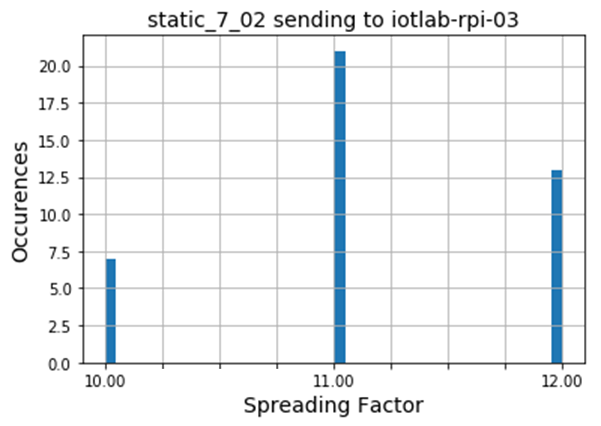
\includegraphics[scale=0.45]{sf_7_02.png}
\caption{SF of the packets received by the Joncquois gateway}
\label{sf_7_02}
\end{figure}

\begin{figure}[htbp]
\centering
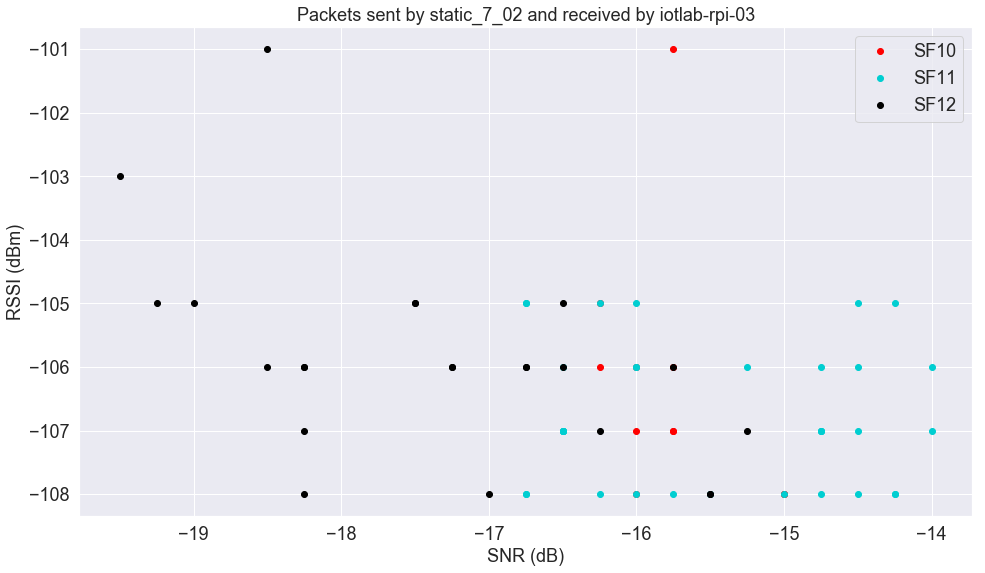
\includegraphics[scale=0.22]{snr_limit.png}
\caption{SNR values of a mediocre transmission}
\label{snr_limit}
\end{figure}

\begin{figure}[htbp]
\centering
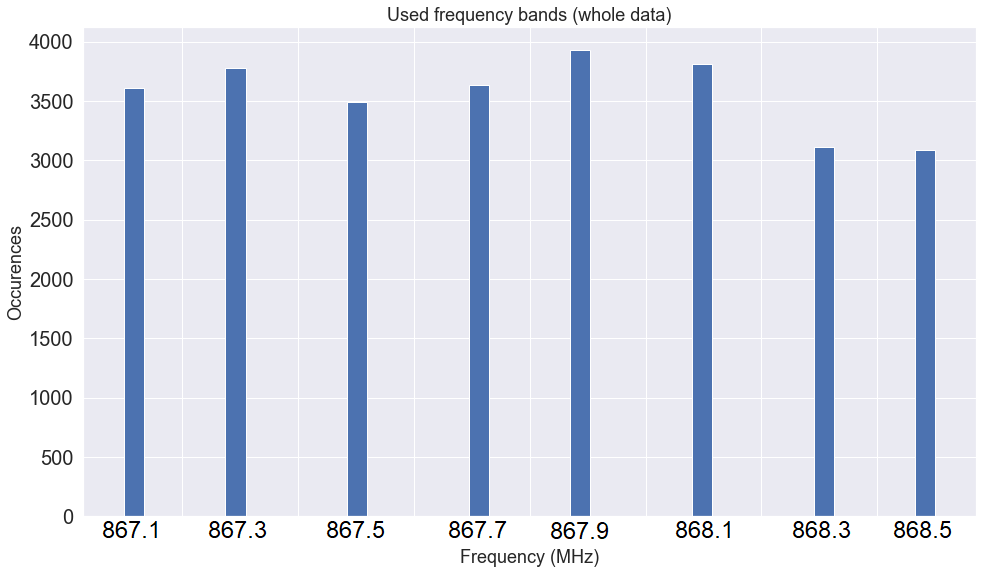
\includegraphics[scale=0.3]{freq_count.png}
\caption{Frequency bands used during the experiment}
\label{freq_count}
\end{figure}

\begin{figure}[htbp]
\centering
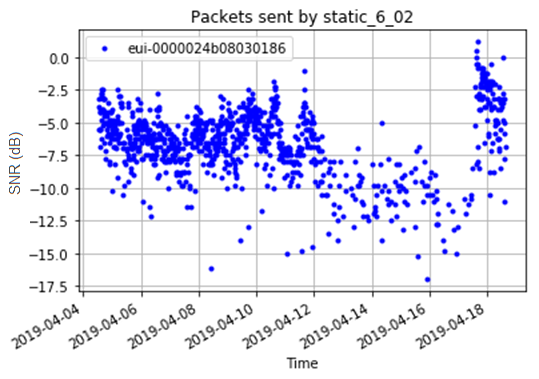
\includegraphics[scale=0.5]{6_02_freq_problem.png}
\caption{Packet delivery drop between the 12.04 and 17.04 (device 6\_02)}
\label{6_02_freq_problem}
\end{figure}

\begin{figure}[htbp]
\centering
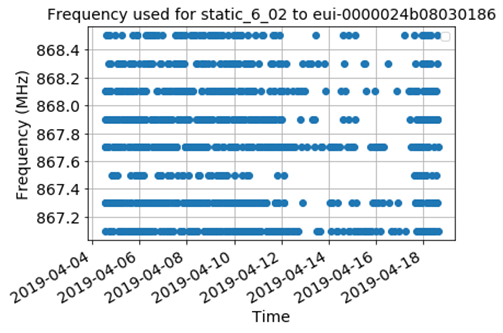
\includegraphics[scale=0.65]{602_freq_bad.png}
\caption{Frequency band used by the device 6\_02 between the 04.04.2019 and 18.04.2019 (Houzeau gateway)}
\label{602_freq}
\end{figure}

\begin{figure}[htbp]
\centering
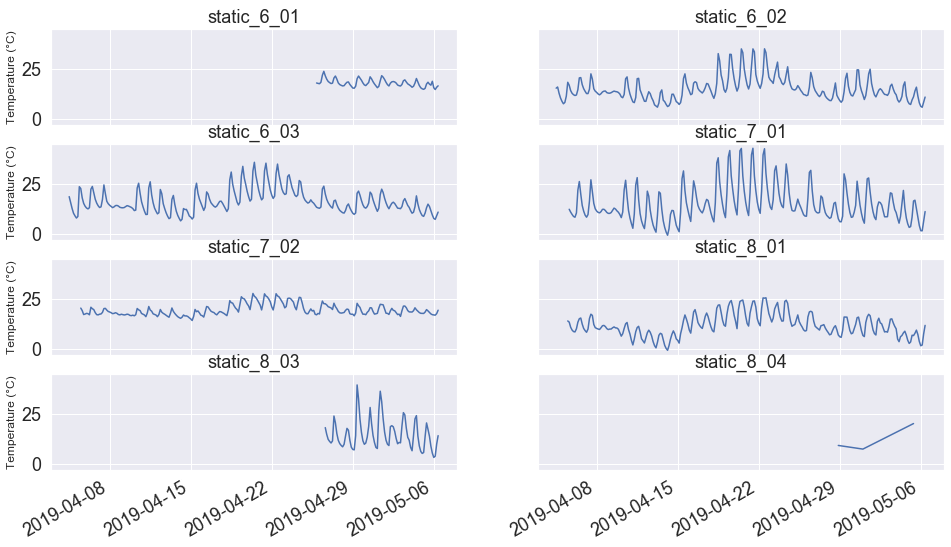
\includegraphics[scale=0.3]{02_temp_all.png}
\caption{Temperature profile on each device (31 days)}
\label{temp_all}
\end{figure}

\begin{figure}[htbp]
\centering
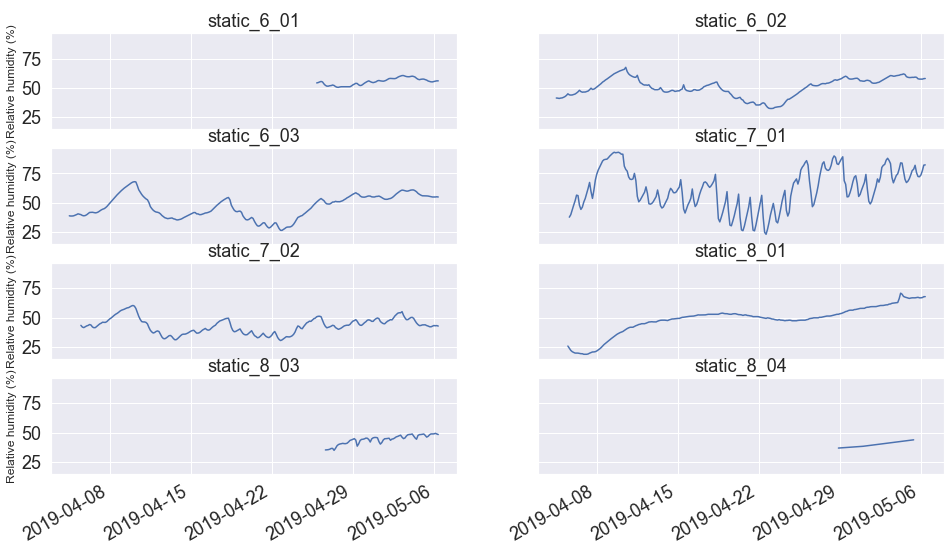
\includegraphics[scale=0.3]{01_rh_all.png}
\caption{RH profile on each device (31 days)}
\label{rh_all}
\end{figure}

\addtolength{\textheight}{-10cm}

\end{document}